%!TEX program = xelatex
% proposal.tex —— 本科毕业设计（论文）开题报告
% 题目：卫星雷达高度计近海回波波形仿真及海洋参数反演误差分析
%
% 版式依据：学校开题报告模板（开题报告（初稿）.doc / .pdf），仿其封面、
%   填写要求页、正文页眉页脚、进度表与封底评审表重排。
% 编译方式：XeLaTeX；无目录，编译一遍即可（有交叉引用改动时编译两遍）。
%
% 骨架说明（撰写阶段内部用，定稿删除）：
%   - 红色批注 \tbd{...} 标注“这一部分写什么、注意事项”，成稿后删除
%   - 各部分素材与论文共用：图 ../Echo_Simulation/output/、../Retracking/output/
%   - 填写要求：理工类 3000 字左右；小四号宋体；A4 双面打印；封面封底浅蓝卡纸
% ---------------------------------------------------------------------------- %

\documentclass[a4paper]{article}

% ---------------------------------- layout ---------------------------------- %
\usepackage[a4paper,top=2.5cm,bottom=2.5cm,left=2.8cm,right=2.8cm,
            headheight=1.2cm,headsep=1em,footskip=1.5em]{geometry}

% ----------------------------------- fonts ---------------------------------- %
% 与 Thesis/thesis.tex 保持一致：Fandol 字族 + Times New Roman
\usepackage{ctex}
\usepackage{xeCJK}
\setCJKmainfont{FandolSong}
\setCJKsansfont{FandolSong}
\setCJKmonofont{FandolSong}
\setCJKfamilyfont{song}{FandolSong}
\newcommand{\song}{\CJKfamily{song}}
\setCJKfamilyfont{kai}{FandolKai}
\newcommand{\kai}{\CJKfamily{kai}}
\setCJKfamilyfont{hwzs}{FandolFang}
\newcommand{\hwzs}{\CJKfamily{hwzs}}
\setCJKfamilyfont{hei}{FandolHei}
\newcommand{\hei}{\CJKfamily{hei}}
\usepackage{fontspec}
\setmainfont{Times New Roman}
\setsansfont{Times New Roman}
\setmonofont{Times New Roman}

% 字号（与论文一致）
\newcommand{\yihao}{\fontsize{26pt}{36pt}\selectfont}
\newcommand{\xiaoerhao}{\fontsize{18pt}{24pt}\selectfont}
\newcommand{\sanhao}{\fontsize{15.75pt}{22pt}\selectfont}
\newcommand{\sihao}{\fontsize{14pt}{20pt}\selectfont}
\newcommand{\xiaosihao}{\fontsize{12pt}{18pt}\selectfont}
\newcommand{\wuhao}{\fontsize{10.5pt}{15pt}\selectfont}

% ---------------------------------- misc ------------------------------------ %
\usepackage{amsmath}
\usepackage{graphicx}
\graphicspath{{./}{../Thesis/}{../Echo_Simulation/output/}{../Retracking/output/}}
\usepackage{xcolor}
\usepackage{array}
\usepackage{multirow}

% 撰写阶段红色批注（定稿删除）
\newcommand{\tbd}[1]{\par{\color{red}\kai\xiaosihao 【TODO】#1}}

% -------------------------------- header/footer ------------------------------ %
% 正文页页眉：华中科技大学本科毕业设计（论文）开题报告；页脚：居中页码
\usepackage{fancyhdr}
\newcommand{\headstyle}{%
  \fancyhead[C]{\hwzs\wuhao 华\hspace{0.4em}中\hspace{0.4em}科\hspace{0.4em}技\hspace{0.4em}大\hspace{0.4em}学\hspace{0.4em}本\hspace{0.4em}科\hspace{0.4em}毕\hspace{0.4em}业\hspace{0.4em}设\hspace{0.4em}计（论\hspace{0.4em}文）开\hspace{0.4em}题\hspace{0.4em}报\hspace{0.4em}告}}
\newcommand{\footstyle}{\fancyfoot[C]{\wuhao\thepage}}
\pagestyle{fancy}
\fancyhf{}
\headstyle
\footstyle
\renewcommand{\headrulewidth}{0.4pt}

% ------------------------------ 正文基本样式 -------------------------------- %
% 正文：小四号宋体，1.5 倍行距，首行缩进 2 字符
\renewcommand{\baselinestretch}{1.5}
\setlength{\parindent}{2em}

% 章节标题：一、二、三…… 小四黑体（与初稿一致，不进目录）
\newcommand{\sect}[1]{\par\vspace{0.8em}{\noindent\hei\xiaosihao #1}\par\vspace{0.3em}}
% 小标题：（一）（二）…… 小四黑体
\newcommand{\subsect}[1]{\par\vspace{0.5em}{\noindent\hei\xiaosihao #1}\par\vspace{0.2em}}

% 封面字段行：#1#2 组成四字宽的分散标签，#3 为下划线上的填充内容
\newcommand{\coverline}[3]{\noindent\makebox[4em][s]{\hfill #1\hfill #2\hfill}\hspace{0.5em}\underline{\makebox[8.8cm][c]{\sanhao #3}}}

% 图表标题样式
\usepackage{float}
\usepackage{caption}
\DeclareCaptionFont{heixiaosi}{\hei\xiaosihao}
\captionsetup[figure]{labelsep=quad,name={图},font=heixiaosi}
\captionsetup[table]{labelsep=quad,name={表},font=heixiaosi}

% 参考文献样式（GB/T 7714 顺序编码制；定稿可用 biblatex 或手工 thebibliography）
\renewcommand{\refname}{\centering\hei\xiaosihao 参考文献}

\begin{document}

% ============================== 封面 ============================== %
\begin{titlepage}
  \begin{center}
    \vspace*{1.2cm}
    
\includegraphics[height=1.6cm]{hust_logo_calligraphy.png}\par
    \vspace{1.2cm}
    {\hei\bfseries\yihao 本科毕业设计（论文）开题报告}\par
    \vspace{2.2cm}
    {\sanhao\bfseries
      \makebox[4em][s]{\hfill 题\hfill 目\hfill}：卫星雷达高度计近海回波波形仿真及\par
      \vspace{0.4em}
      海洋参数反演误差分析\par}
    \vspace{2.6cm}
    {\sanhao
      \coverline{院}{系}{电子信息与通信学院}\par\vspace{0.9em}
      \coverline{专}{业}{电信2203班}\par\vspace{0.9em}
      \coverline{姓}{名}{蒲奕帆}\par\vspace{0.9em}
      \coverline{学}{号}{U202213789}\par\vspace{0.9em}
      \coverline{指导教师}{}{田加胜}\par}
    \vfill
    {\sanhao 2026 年 2 月 28 日\par}
    \vspace{1.5cm}
  \end{center}
\end{titlepage}

% ============================ 填写要求页 =========================== %
\thispagestyle{empty}
\begin{center}
  {\hei\sihao 开题报告填写要求}
\end{center}
\vspace{1em}
{\song\xiaosihao
\noindent 一、开题报告主要内容：\par
1.课题来源、目的、意义。\par
2.国内外研究现况及发展趋势。\par
3.预计达到的目标、关键理论和技术、主要研究内容、完成课题的方案及主要措施。\par
4.课题研究进度安排。\par
5.主要参考文献。\par
\noindent 二、报告内容用小四号宋体字编辑，采用A4号纸双面打印，封面与封底采用浅蓝色封面纸（卡纸）打印。要求内容明确，语句通顺。\par
\noindent 三、指导教师评语、教研室（系、所）或开题报告答辩小组审核意见用蓝、黑钢笔手写或小四号宋体字编辑，签名必须手写。\par
\noindent 四、理、工、医类要求字数在3000字左右，文、管类要求字数在2000字左右。\par
\noindent 五、开题报告应在第八学期第二周之前完成。\par}

% ============================== 正文 ============================== %
\clearpage
\setcounter{page}{1}

% -------- 一、课题来源、目的、意义 -------- %
\sect{一、课题来源、目的、意义}
\tbd{写什么：课题来源（导师拟定／自选，结合近海测高这一背景）；研究目的（近海波形仿真模型＋重跟踪优化＋误差源定量分析）；研究意义（理论：近海回波建模与误差分析体系；应用：风浪监测、海平面变化、灾害预警的数据支撑）。约 500--600 字，可参考初稿第一部分并按论文最终口径修改。}

% -------- 二、国内外研究现况及发展趋势 -------- %
\sect{二、国内外研究现况及发展趋势}
\tbd{写什么：国外——Brooks 阈值重构、Deng 波形分类与多阈值、ALBICOCCA／ALTICORE／COASTALT／PISTACH 项目、Lefevre 双参数风速反演、Tournadre 目标探测；国内——鲍李峰 5-$\beta$＋OCOG、Guo 改进阈值、赵健对比重构、杨乐波形分类子波形、神经网络四参数风速反演、“构造波形”方法；发展趋势——近海不可用距离从 20 km 缩至 5 km、SWH 误差 0.2 m 内、风速 RMSE 优于 1.3 m/s，仍有复杂校正量获取与海陆复合散射仿真待突破。约 800--900 字。}

% -------- 三、预计达到的目标、关键理论和技术、主要研究内容、方案及措施 -------- %
\sect{三、预计达到的目标、关键理论和技术、主要研究内容、完成课题的方案及主要措施}
\tbd{写什么：这是篇幅最大的一编部分（约 1200--1500 字），建议分（一）（二）（三）（四）小节，与论文章节对应：}

\subsect{（一）预计达到的目标}
\tbd{定量目标：完成近海回波仿真平台；重跟踪反演精度指标（SWH RMSE、风速 RMSE、近岸可用距离）；误差源识别与校正方案。}

\subsect{（二）关键理论和技术：海面建模与后向散射系数计算}
\tbd{二维 PM 谱＋FFT/Monte-Carlo 生成粗糙海面；KA（Kirchhoff 近似）计算后向散射系数。公式示例（定稿替换为最终公式组）：}
% 公式示例：
% \begin{equation}
%   \sigma^0=\frac{\rho}{\pi\sqrt{\sigma_u^2\sigma_c^2}}\;p(\tan\theta,0)
% \end{equation}

\subsect{（三）关键理论和技术：回波波形仿真}
\tbd{雷达系统参数（轨道高度 1336 km、Ku 波段 13.58 GHz、波束宽度 2.2°、采样频率 320 MHz）；基于雷达方程的面元散射功率叠加生成波形；不同风速下波形特征差异。插图示例（定稿启用）：}
% \begin{figure}[H]
%   \centering
%   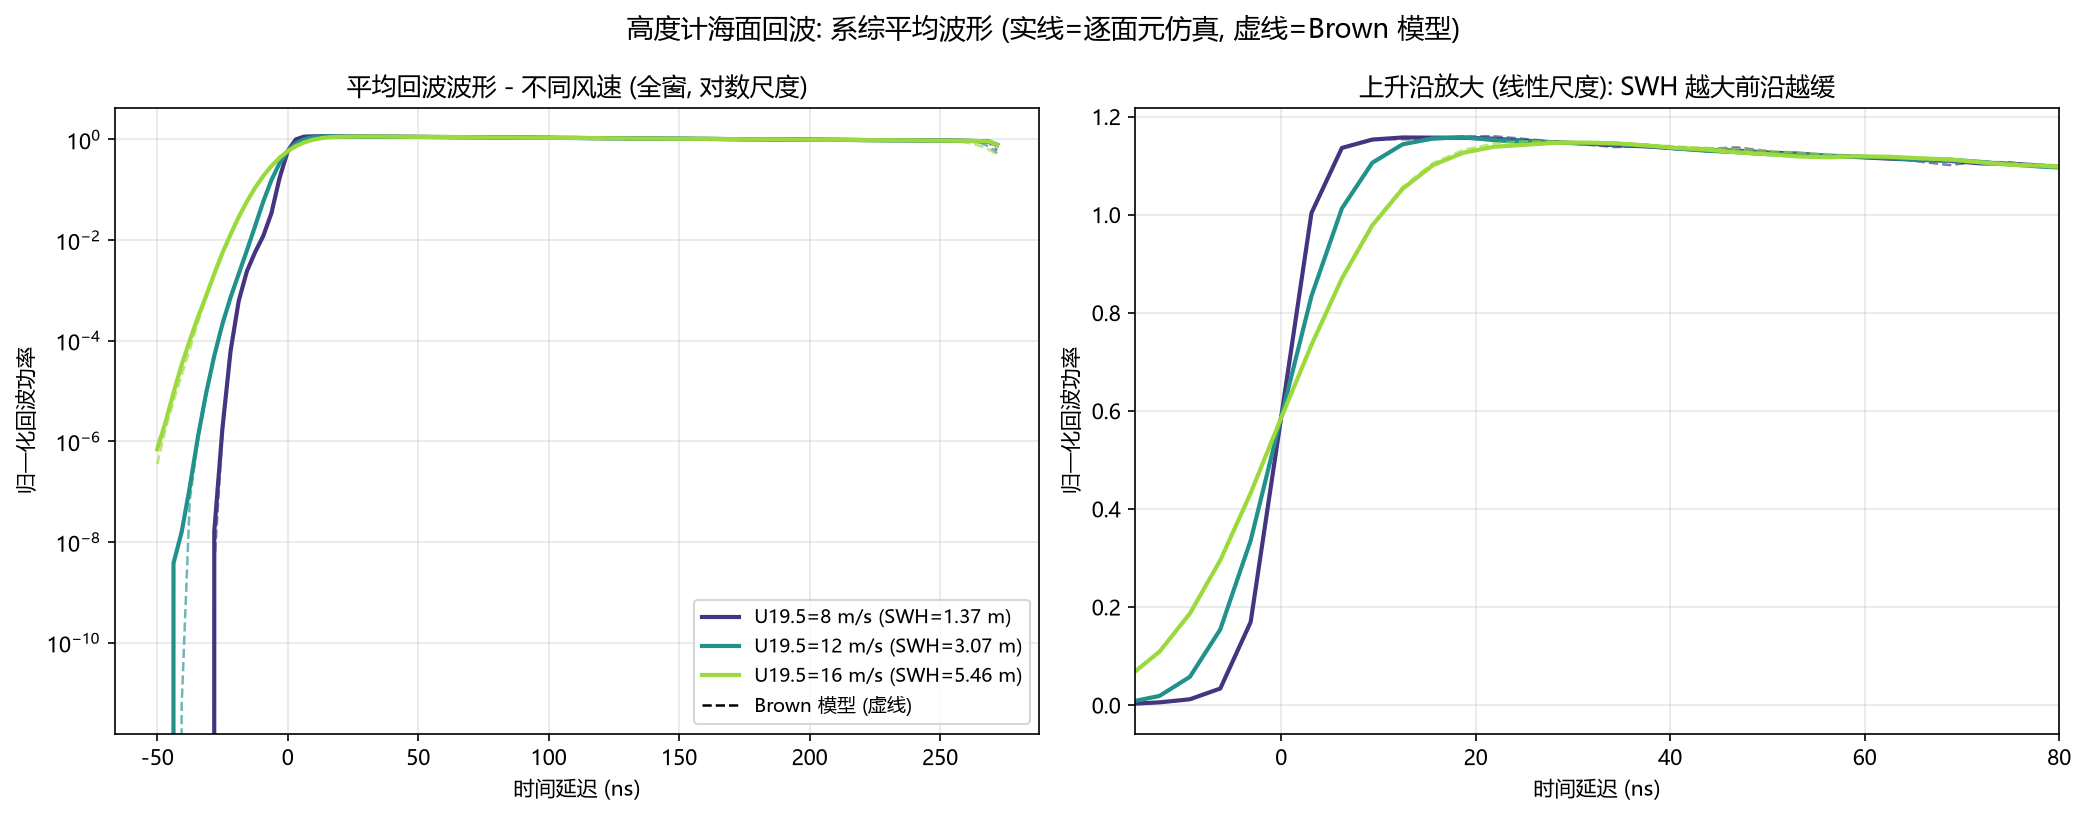
\includegraphics[width=0.8\textwidth]{echo_wind_family.png}
%   \caption{不同风速下的仿真回波波形}
% \end{figure}

\subsect{（四）主要研究内容、完成课题的方案及主要措施}
\tbd{近海参数（风速、SWH、盐度）变化与陆地干扰对回波的影响；“实测—仿真—理论”三方对比的误差分析方法（RMSE／Bias／相关系数）；误差分级校正策略与措施（进度保障、数据来源：Jason-3 SGDR、OIFD 融合 SWH、浮标）。}

% -------- 四、课题研究进度安排 -------- %
\sect{四、课题研究进度安排}
\tbd{下表沿用初稿的进度；若答辩时间线有调整，开学后按新的周次修改。}
\begin{table}[H]
  \centering
  \xiaosihao
  \begin{tabular}{|c|c|p{8.2cm}|}
    \hline
    学期 & 周次 & \multicolumn{1}{c|}{工作任务} \\
    \hline
    \multirow{2}{*}{\shortstack{2025--2026\\学年度\\第一学期}}
      & 19 周——20 周 & 收集参考文献，准备前期工作 \\ \cline{2-3}
      & 20 周——21 周 & 对部分外文参考文献进行翻译 \\ \hline
    \multirow{5}{*}{\shortstack{2025--2026\\学年度\\第二学期}}
      & 1 周——2 周 & 对粗糙海洋表面各类谱进行仿真 \\ \cline{2-3}
      & 3 周——5 周 & 对海洋表面后向散射系数进行仿真 \\ \cline{2-3}
      & 6 周——8 周 & 对海洋表面不同风速下雷达高度计近海回波进行仿真 \\ \cline{2-3}
      & 9 周——11 周 & 对近海仿真结果进行海洋参数反演误差分析 \\ \cline{2-3}
      & 12 周——15 周 & 整理所有资料和研究成果并成文 \\ \hline
  \end{tabular}
  \par\vspace{0.5em}
  {\hei\xiaosihao 表 1\quad 课题研究进度安排表}
\end{table}

% -------- 五、主要参考文献 -------- %
\sect{五、主要参考文献}
\tbd{按 GB/T 7714 顺序编码制列 8--15 条：学位论文（徐浩、杨乐、米银霞、展艺华）＋经典外文（Brown 1977、Hayne 1980、Tsang 散射、Deng 2006 等）。初稿仅 6 条，建议补充 Brown 1977 与近两年文献。}
% \begin{thebibliography}{9}\setlength{\itemsep}{0pt}
%   \small
%   \bibitem{xuhao2020} 徐浩. 基于电磁散射特性的雷达高度计回波仿真与分析[D]. 武汉: 华中科技大学, 2020.
%   \bibitem{hayne1980} Hayne G S. Radar altimeter mean return waveforms from near-normal-incidence ocean surface scattering[J]. IEEE Transactions on Antennas and Propagation, 1980, 28(5): 687-692.
% \end{thebibliography}

% ============================ 封底：评审表 ========================== %
% 标题与表格必须同页：局部收紧行距，单元格高度经过试算避免跨页
\clearpage
\pagestyle{empty}
{\linespread{1.15}\selectfont
\begin{center}
  {\hei\bfseries\sanhao 华中科技大学本科毕业设计（论文）开题报告评审表}
\end{center}
\vspace{0.5em}
\begin{center}
  \xiaosihao
  \begin{tabular}{|>{\centering\arraybackslash}p{1.6cm}|p{2.9cm}|>{\centering\arraybackslash}p{1.6cm}|p{2.9cm}|>{\centering\arraybackslash}p{2.2cm}|p{2.9cm}|}
    \hline
    姓名 & & 学号 & & 指导教师 & \\ \hline
    院（系）专业 & \multicolumn{5}{p{12.5cm}|}{} \\ \hline
    \multicolumn{6}{|p{14.9cm}|}{
      \centering\hei\bfseries 指导教师评语\par\vspace{0.2em}
      \song\raggedright
      1. 学生前期表现情况。\par
      2. 是否具备开始毕业设计（论文）条件？是否同意开始毕业设计（论文）？\par
      3. 不足及建议。\par
    } \\ \hline
    \multicolumn{6}{|p{14.9cm}|}{\vspace{0pt}
      \vspace{6.6cm}
      \par\hfill 指导教师（签名）：\hspace{3em}\par
      \vspace{0.5em}
      \hfill \makebox[9em][s]{\hfill 年\hfill 月\hfill 日\hfill}\hspace{1em}\par
    } \\ \hline
    \multicolumn{6}{|p{14.9cm}|}{
      \centering\hei\bfseries 教研室（系、所）或开题报告答辩小组审核意见\par
    } \\ \hline
    \multicolumn{6}{|p{14.9cm}|}{\vspace{0pt}
      \vspace{5.2cm}
      \par\hfill 教研室（系、所）或开题报告答辩小组负责人（签名）：\hspace{3em}\par
      \vspace{0.5em}
      \hfill \makebox[9em][s]{\hfill 年\hfill 月\hfill 日\hfill}\hspace{1em}\par
    } \\ \hline
  \end{tabular}
\end{center}
}

\end{document}
